\section{Autômatos finitos}

\begin{frame}[fragile]{Reconhecedores}

    \begin{itemize}
        \item Um reconhecedor é um programa que identifica, respondendo \code{cpp}{"Sim"} ou \code{cpp}{"Nao"}, se uma cadeia é ou não uma sentença válida de uma
            determinada linguagem
        \pause

        \item Uma estratégia para a compilação de expressões regulares em reconhecedores é o uso de diagramas de transição generalizados, denominados autômatos
            finitos
        \pause

        \item Um autômato finito pode ser determinístico ou não-determinístico: no segundo caso, podem exister duas ou mais transições com o mesmo rótulo partindo
            de um mesmo estado
        \pause

        \item Autômatos determinísticos podem resultar em reconhecimentos mais rápidos do que os não-determinísticos, porém em geral são muito maiores, no
            que diz respeito ao número de estados e transições
        \pause

        \item É possível representar expressões regulares em ambos tipos de autômatos finitos
    \end{itemize}

\end{frame}

\begin{frame}[fragile]{Autômatos finitos não-determinísticos}

    \begin{block}{Definição de AFN}
        Um autômato finito não-determinístico (AFN) é um modelo matemático que consiste em
        \begin{enumerate}
            \item um conjunto de estados $S$,

            \item um alfabeto $\Sigma$ de símbolos de entrada,

            \item uma função de transição que mapeia pares (estado, símbolo) em um conjunto de estados,

            \item um estado $s_0$, denominado estado inicial ou de partida, e

            \item um conjunto $F$ de estados de aceitação (ou estados finais).
        \end{enumerate}
    \end{block}

\end{frame}

\begin{frame}[fragile]{Grafo de transições}

    \begin{itemize}
        \item Um AFN pode ser representado por meio de um grafo direcionado e rotulado, denominado grafo de transição
        \pause

        \item Em um grafo de transição, os nós representam os estados e as arestas definem a função de transição
        \pause

        \item Os rótulos das arestas são os símbolos associados à transição, e a direção da aresta parte do estado atual para o próximo estado
        \pause

        \item Grafos de transição se assemelham aos diagramas de transição, com duas diferenças fundamentais
        \pause

        \item A primeira diferença é que um mesmo rótulo pode estar associado a duas ou mais arestas partindo de um mesmo estado
        \pause

        \item A segunda é que o símbolo \code{apl}{∊} pode rotular uma aresta
    \end{itemize}

\end{frame}

\begin{frame}[fragile]{Grafo de transição para a linguagem $(a\ |\ b)^*abb$}

    \begin{figure}
        \centering

        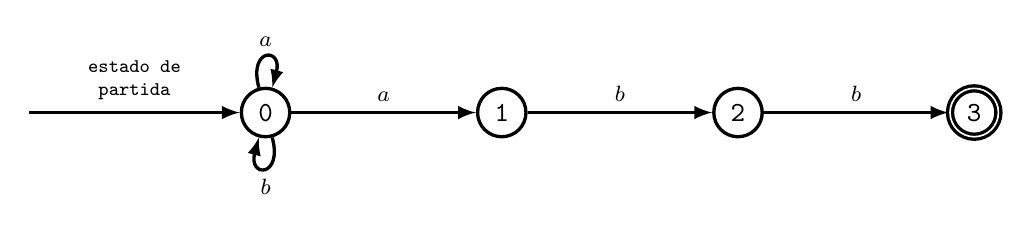
\begin{tikzpicture} 
            \coordinate (X) at (0, 6);

            \node[draw,circle,very thick] (A0) at (3, 6) { \texttt{0} };
            \node[draw,circle,very thick] (A1) at (6, 6) { \texttt{1} };
            \node[draw,circle,very thick] (A2) at (9, 6) { \texttt{2} };
            \node[draw,circle,double,very thick] (A3) at (12, 6) { \texttt{3} };

            \draw[very thick,-latex] (X) to node[above] { \scriptsize \texttt{\begin{tabular}{c}estado de\\ partida\end{tabular}} } (A0);
            \draw[very thick,-latex] (A0) to node[above] { \footnotesize $a$ } (A1);
            \draw[very thick,-latex] (A1) to node[above] { \footnotesize $b$ } (A2);
            \draw[very thick,-latex] (A2) to node[above] { \footnotesize $b$ } (A3);
            \draw[very thick,-latex] (A0) to [loop above] node[above] { \footnotesize $a$ } (A0);
            \draw[very thick,-latex] (A0) to [loop below] node[below] { \footnotesize $b$ } (A0);

        \end{tikzpicture} 
    \end{figure}
\end{frame}

\begin{frame}[fragile]{Tabela de transições}

    \begin{itemize}
        \item Uma alternativa para a implementação da função de transição é a tabela de transições
        \pause

        \item Em uma tabela de transições cada linha representa um estado e cada coluna representa um rótulo
        \pause

        \item Se necessário, é necessário adicionar uma coluna para o rótulo \code{apl}{∊}
        \pause

        \item A entrada da tabela posicionada na línha $i$, coluna $c$, contém o conjunto de estados que podem suceder o estado $i$ quando o caractere $c$
            for lido na entrada
        \pause

        \item De fato, a tabela de transições corresponde à representação do grafo de transições como uma matriz de adjacências
        \pause

        \item Outra alternativa é representar o grafo por meio de uma lista de adjacências
    \end{itemize}

\end{frame}

\begin{frame}[fragile]{Tabela de transições do AFN da linguagem $(a\ |\ b)^*abb$}

    \begin{table}
        \centering

        \begin{tabular}{ccc}
        \toprule
        \multirow{2}{*}{\textbf{Estado}} & \multicolumn{2}{c}{\textbf{Símbolo de entrada}} \\
        & $a$ & $b$ \\ 
        \midrule
        \texttt{0} & \texttt{\{ 0, 1 \}} & \texttt{\{ 0 \}} \\
        \texttt{1} & \texttt{-} & \texttt{\{ 2 \}} \\
        \texttt{2} & \texttt{-} & \texttt{\{ 3 \}} \\
        \bottomrule
        \end{tabular}
    \end{table}

\end{frame}

\begin{frame}[fragile]{Caminhos}

    \begin{itemize}
        \item Um caminho em um grafo de transições é uma sequência de arestas de transição
        \pause

        \item Os rótulos das arestas, quando concatenados, formam uma cadeia $s$
        \pause

        \item Caso o símbolo \code{apl}{∊} seja o rótulo de uma ou mais arestas de um caminho, na concatenação dos rótulos este símbolo é descartado
        \pause

        \item Um AFN aceita uma cadeia de entrada $s$ se, e somente se, existe um caminho no grafo de transições que parte do estado inicial e que termina em 
            algum estado de aceitação
        \pause

        \item Pode existir mais de um caminho que leva a um estado de aceitação
        \pause

        \item A linguagem definida por um AFN é o conjunto de cadeias que são aceitas
    \end{itemize}

\end{frame}

\begin{frame}[fragile]{AFN da linguagem $aa^*\ |\ bb^*$}

    \begin{figure}
        \centering

        \begin{tikzpicture} 
            \coordinate (X) at (0, 4);
            \node[opacity=0] (0, 0) { };

            \node[draw,circle,very thick] (A0) at (3, 4) { \texttt{0} };
            \node[draw,circle,very thick] (A1) at (6, 6) { \texttt{1} };
            \node[draw,circle,double,very thick] (A2) at (9, 6) { \texttt{2} };
            \node[draw,circle,very thick] (A3) at (6, 2) { \texttt{3} };
            \node[draw,circle,double,very thick] (A4) at (9, 2) { \texttt{4} };

            \draw[very thick,-latex] (X) to node[above] { \scriptsize \texttt{\begin{tabular}{c}estado de\\ partida\end{tabular}} } (A0);
            \draw[very thick,-latex] (A0) to node[above] { \footnotesize \code{apl}{∊} } (A1);
            \draw[very thick,-latex] (A0) to node[above] { \footnotesize \code{apl}{∊} } (A3);
            \draw[very thick,-latex] (A1) to node[above] { \footnotesize $a$ } (A2);
            \draw[very thick,-latex] (A3) to node[above] { \footnotesize $b$ } (A4);
            \draw[very thick,-latex] (A2) to [loop right] node[right] { \footnotesize $a$ } (A2);
            \draw[very thick,-latex] (A4) to [loop right] node[right] { \footnotesize $b$ } (A4);

        \end{tikzpicture} 
    \end{figure}
\end{frame}

\begin{frame}[fragile]{AFN da linguagem $aa^*\ |\ bb^*$}

    \begin{figure}
        \centering

        \begin{tikzpicture} 
            \coordinate (X) at (0, 4);
            \node[opacity=0] (0, 0) { pqgh };

            \node[draw,circle,very thick] (A0) at (3, 4) { \texttt{0} };
            \node[draw,circle,very thick] (A1) at (6, 6) { \texttt{1} };
            \node[draw,circle,double,very thick] (A2) at (9, 6) { \texttt{2} };
            \node[draw,circle,very thick] (A3) at (6, 2) { \texttt{3} };
            \node[draw,circle,double,very thick] (A4) at (9, 2) { \texttt{4} };

            \draw[very thick,-latex] (X) to node[above] { \scriptsize \texttt{\begin{tabular}{c}estado de\\ partida\end{tabular}} } (A0);
            \draw[very thick,-latex] (A0) to node[above] { \footnotesize \code{apl}{∊} } (A1);
            \draw[very thick,-latex] (A0) to node[above] { \footnotesize \code{apl}{∊} } (A3);
            \draw[very thick,-latex] (A1) to node[above] { \footnotesize $a$ } (A2);
            \draw[very thick,-latex] (A3) to node[above] { \footnotesize $b$ } (A4);
            \draw[very thick,-latex] (A2) to [loop right] node[right] { \footnotesize $a$ } (A2);
            \draw[very thick,-latex] (A4) to [loop right] node[right] { \footnotesize $b$ } (A4);

            \node[anchor=west] at (0.2, 0.2) { \footnotesize \texttt{\begin{tabular}{cc}Caminho que aceita\\ a cadeia $aa$\end{tabular}} };
            \node (B0) at (4.5, 0.2) { \footnotesize 0 };
            \node (B1) at (6.0, 0.2) { \footnotesize 1 };
            \node (B2) at (7.5, 0.2) { \footnotesize 2 };
            \node (B3) at (9.0, 0.2) { \footnotesize 2 };


            \draw[very thick,-latex] (B0) to node[above] { \footnotesize \code{apl}{∊} } (B1);
            \draw[very thick,-latex] (B1) to node[above] { \footnotesize $a$ } (B2);
            \draw[very thick,-latex] (B2) to node[above] { \footnotesize $a$ } (B3);

        \end{tikzpicture} 
    \end{figure}
\end{frame}

\begin{frame}[fragile]{Autômatos finitos determinísticos}

    \begin{block}{Definição de AFD}
        Um autômato finito deerminístico (AFD) é um caso especial de AFN no qual
        \begin{enumerate}
            \item nenhum estado possui um transição rotulada pelo símbolo \code{apl}{∊} (denominada transição-\code{apl}{∊}); e
            \item para cada estado $s$ existe no máximo uma transição rotulada com o caractere $c$ partindo de $s$.
        \end{enumerate}
    \end{block}

    \vspace{0.2in}

    Observação: em um AFD, cada entrada da tabela de transições contém um único estado, o que simplifica o processo de verificação de aceitação de uma cadeia.
\end{frame}

\begin{frame}[fragile]{Pseudocódigo para verificação de cadeias por meio de um AFD}

    \begin{algorithmic}[1]
        \Require{Uma cadeia de entrada $x$ terminada por um \code{cpp}{EOF}}
        \Ensure{\code{cpp}{"Sim"}, caso a cadeia seja uma sentença válida da linguagem, ou \code{cpp}{"Nao"}, caso contrário}
        \vspace{0.2in}
        \State{$s\gets s_0$}
        \State{$c\gets \Call{próximoCaractere}{\,}$}
        \Statex
        \While{$c\neq \code{cpp}{EOF}$ }
            \State{$s\gets$ \Call{transição}{$s, c$}}
            \State{$c\gets \Call{próximoCaractere}{\,}$}
        \EndWhile
        \Statex
        \If{$s\in F$}
            \State \Return{\code{cpp}{"Sim"}}
        \Else
            \State \Return{\code{cpp}{"Não"}}
        \EndIf
    \end{algorithmic}

\end{frame}
